\documentclass[10pt, compress, aspectratio=169]{beamer}

\usetheme[numbering=fraction, progressbar=none, titleformat=smallcaps]{metropolis}
\usepackage{booktabs}
\usepackage{array}
\usepackage{listings}
\usepackage{graphicx}
\usepackage[scale=2]{ccicons}
\usepackage{url}
\usepackage{relsize}
\usepackage{wasysym}

\usepackage{pgfplots}
\usepgfplotslibrary{dateplot}

\lstset{ %
  backgroundcolor={},
  basicstyle=\ttfamily\footnotesize,
  breakatwhitespace=true,
  breaklines=true,
  captionpos=n,
  commentstyle=\color{orange},
  escapeinside={\%*}{*)},
  extendedchars=true,
  frame=n,
  keywordstyle=\color{orange},
  language=bash,
  rulecolor=\color{black},
  showspaces=false,
  showstringspaces=false,
  showtabs=false,
  numbers=left,
  numbersep=3pt,
  stepnumber=1,
  stringstyle=\color{gray},
  tabsize=2,
  keywords={thrust,plus,device_vector, copy,transform,begin,end, copyin,
  copyout, acc, \_\_global\_\_, void, int, float, main, threadIdx, blockIdx,
  blockDim, if, else, malloc, NULL, cudaMalloc, cudaMemcpy, cudaSuccess,
  cudaGetLastError, cudaDeviceSynchronize, cudaFree, cudaMemcpyDeviceToHost,
  cudaMemcpyHostToDevice, const, data, independent, kernels, loop,
  fprintf, stderr, cudaGetErrorString, EXIT_FAILURE, for, dim3},
  otherkeywords={::, \#pragma, \#include, <<<,>>>, \&, \*, +, -, /, [, ], >, <}
}

\renewcommand*{\UrlFont}{\ttfamily\smaller\relax}

\graphicspath{{images/}}

\title{Basic Shell}
\author{\footnotesize Rodrigo Siqueira \\ {\scriptsize siqueira@ime.usp.br}}
%\institute{
\includegraphics[height=2cm]{imelogo}\\[0.2cm] Department of Computer Science \\ University of São Paulo}

\begin{document}

\maketitle

%------------------------------------------------------------------------------
\section{Introduction}
\begin{frame}{Overview}
  \begin{figure}
    \centering
    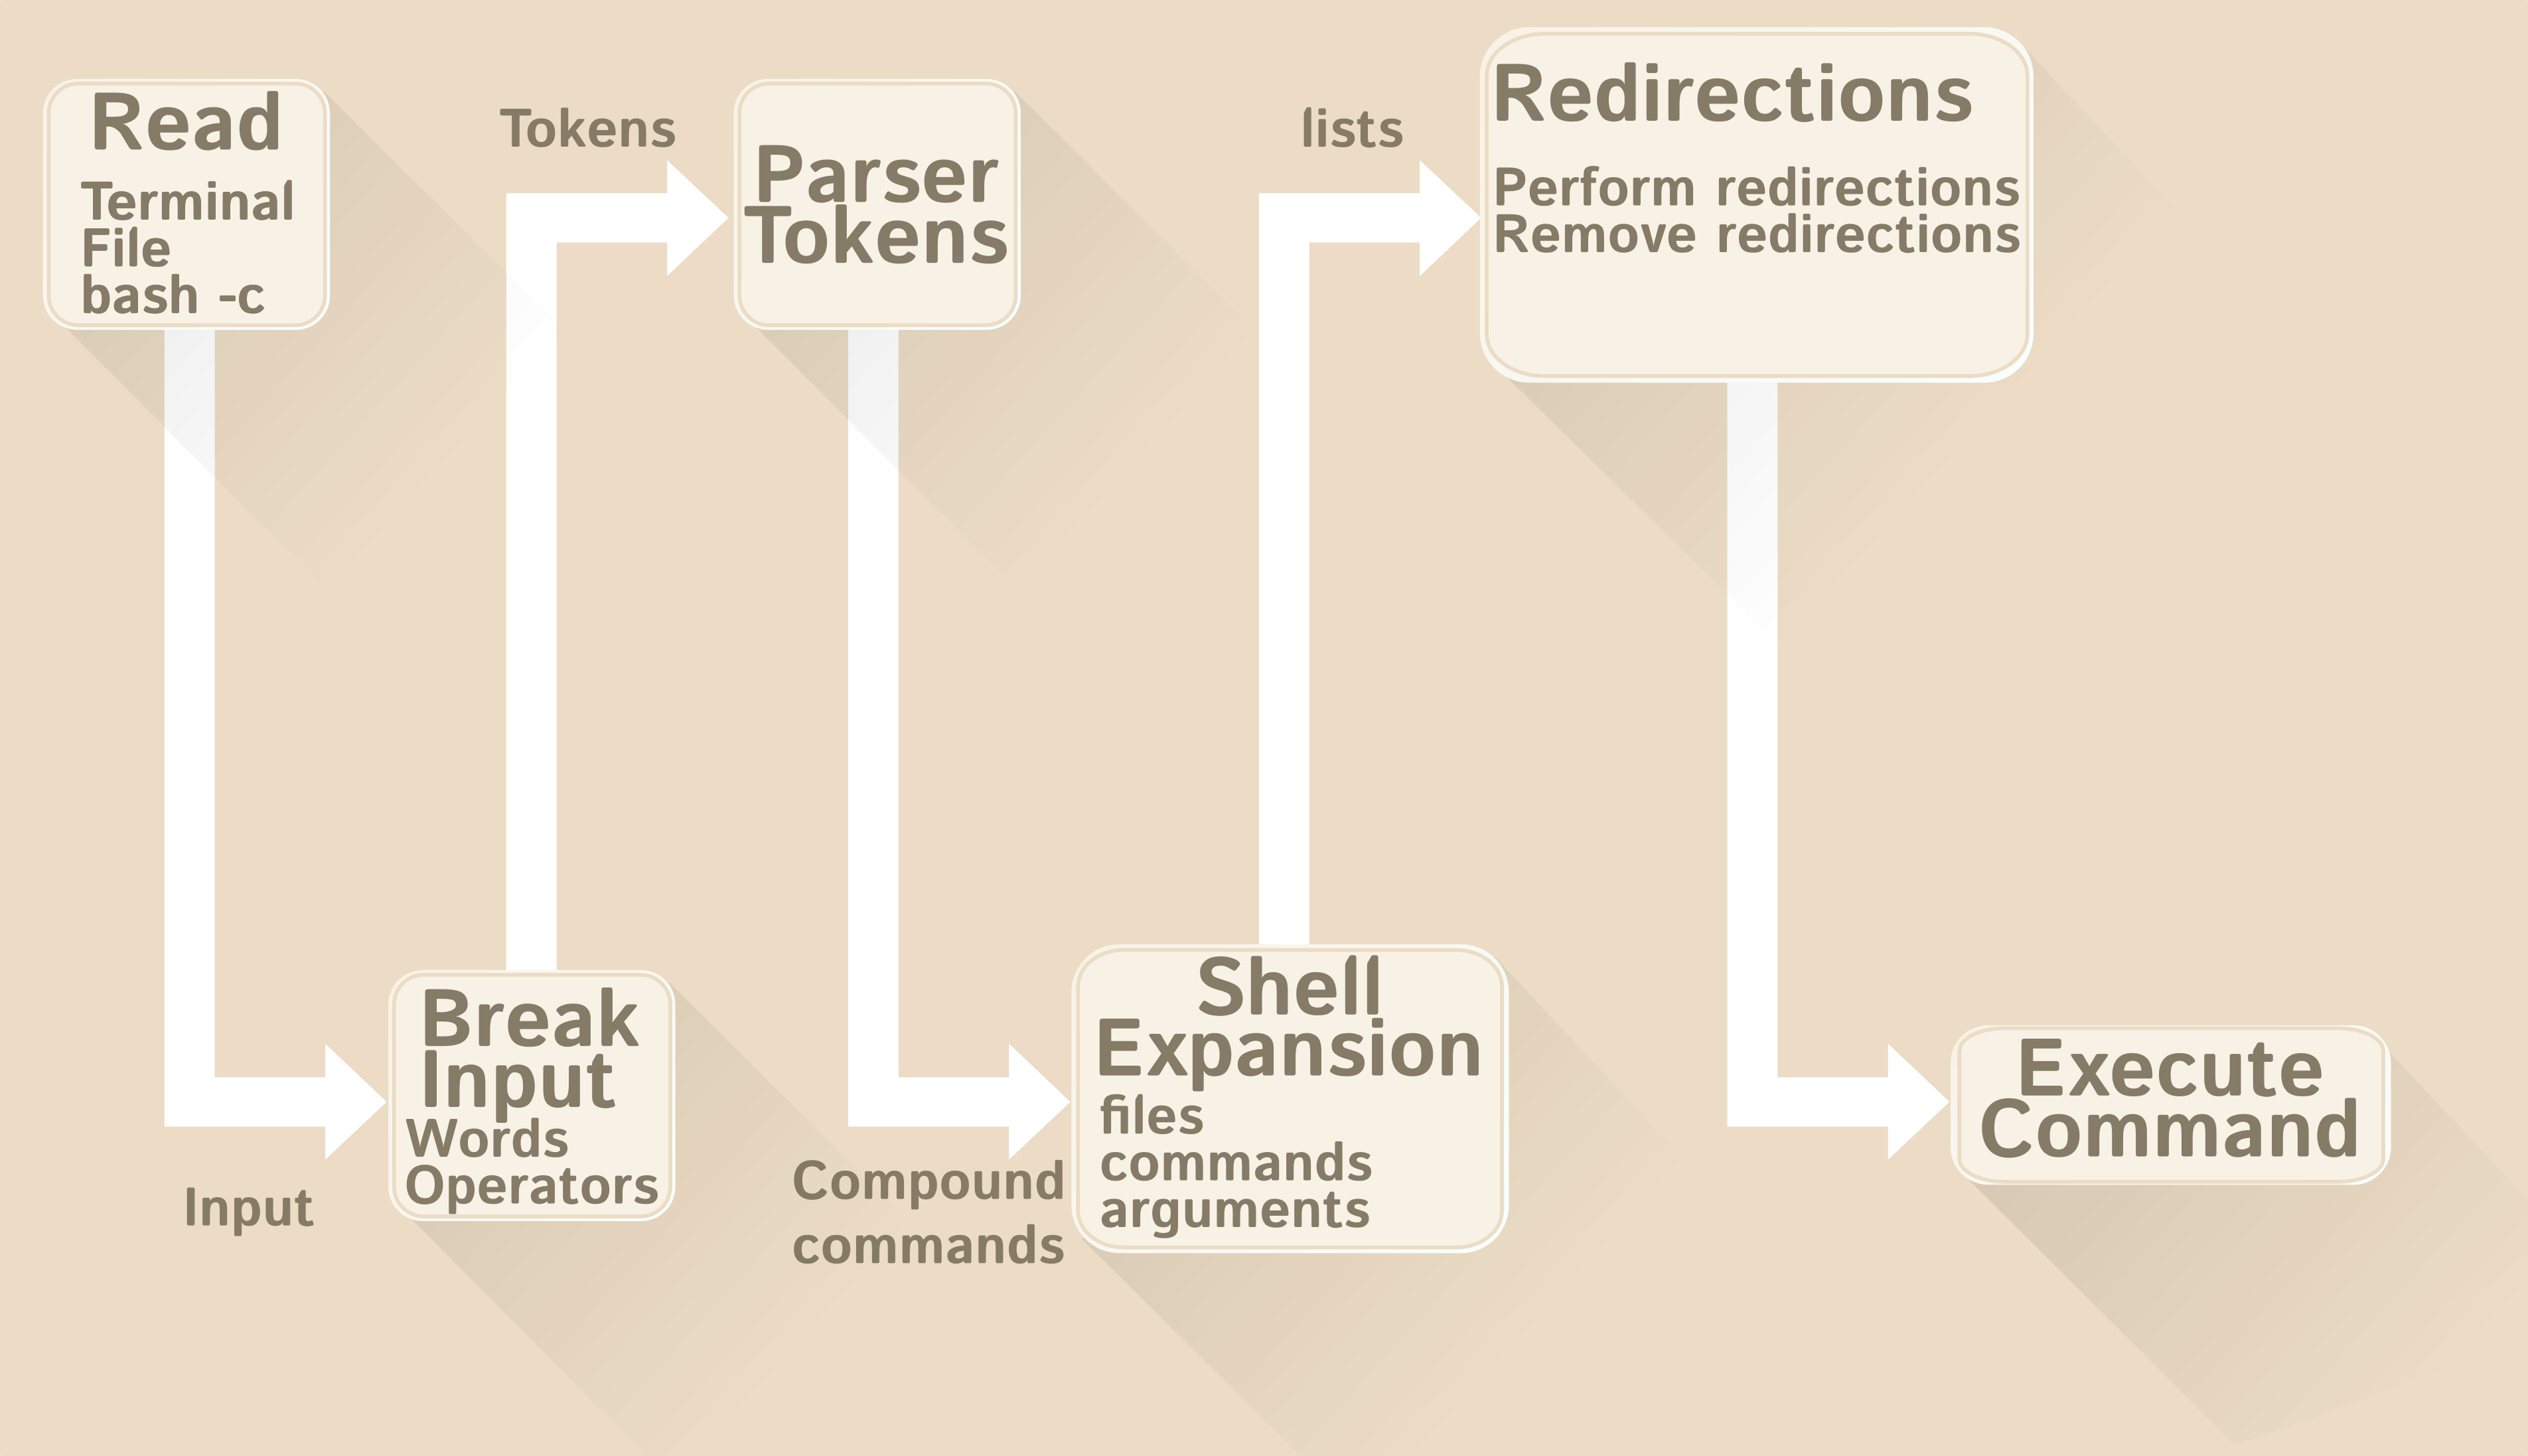
\includegraphics[width=\linewidth,
                     height=0.8\textheight,
                     keepaspectratio]{shell_operations}
    \caption{Shell Operation}
  \end{figure}
\end{frame}

%------------------------------------------------------------------------------
\section{Break Input}

\begin{frame}{Quoting}
  \metroset{block=fill}
  \begin{exampleblock}{About}
    \begin{itemize}
      \item Single Quotes (' ')
      \item Double Quotes (" "): \$, ', and \textbackslash
      \item Escape Character (\textbackslash)
    \end{itemize}
  \end{exampleblock}
\end{frame}

%------------------------------------------------------------------------------
\section{Parser Tokens}

\begin{frame}{Pipelines}
  \metroset{block=fill}
  \begin{exampleblock}{About}
    \begin{itemize}
      \item Connect commands
      \item Performed before any redirection
      \item \textcolor{red}{\texttt{|}} or \textcolor{red}{\texttt{|\&}}
      \item Each command in a pipeline is executed in its own subshell
    \end{itemize}
  \end{exampleblock}
\end{frame}

\begin{frame}{Lists of Commands}
  \metroset{block=fill}
  \begin{exampleblock}{About}
    \begin{itemize}
      \item \textbf{\texttt{\&\&}}
      \item \textbf{\texttt{||}}
      \item \textbf{\texttt{;}}
      \item \textbf{\texttt{\&}}
    \end{itemize}
  \end{exampleblock}
  Examples: \\
  \texttt{command1 \&\& command2} \\
  \texttt{command1 || command2} \\
  \texttt{command1; command2}
\end{frame}

\begin{frame}{Compound Commands: Looping Constructor (\texttt{until})}
  \metroset{block=fill}
  \begin{alertblock}{Syntax}
    \texttt{\textbf{\textcolor{orange}{until}} test-commands;
            \textbf{\textcolor{orange}{do}}
            consequent-commands; \textbf{\textcolor{orange}{done}}}
  \end{alertblock}
  \begin{exampleblock}{About}
    \begin{itemize}
      \item Attention to the spaces, they are part of the syntax
      \item Return: it is the status of the last command executed
    \end{itemize}
  \end{exampleblock}
\end{frame}

\begin{frame}{Compound Commands: Looping Constructor (\texttt{until})}
  \metroset{block=fill}
  \lstinputlisting{codes/stop_and_go.sh}
  Example: \\
  \texttt{./stop\_and\_go.sh green blue red gray}
\end{frame}

\begin{frame}{Compound Commands: Looping Constructor (\texttt{while})}
  \metroset{block=fill}
  \begin{alertblock}{Syntax}
    \texttt{\textbf{\textcolor{orange}{while}} test-commands;
            \textbf{\textcolor{orange}{do}}
            consequent-commands; \textbf{\textcolor{orange}{done}}}
  \end{alertblock}
  \begin{exampleblock}{About}
    \begin{itemize}
      \item Repeats the commands, until the test become different of zero
      \item Return: it is the status of the last command executed
    \end{itemize}
  \end{exampleblock}
\end{frame}

\begin{frame}{Compound Commands: Looping Constructor (\texttt{while})}
  \metroset{block=fill}
  \lstinputlisting{codes/open_3_terminals.sh}
\end{frame}

\begin{frame}{Compound Commands: Looping Constructor (\texttt{for})}
  \metroset{block=fill}
  \begin{alertblock}{Syntax}
    \texttt{\textbf{\textcolor{orange}{for}} [ [ \textbf{\textcolor{orange}{in}}
            [words ...] ] ; ];
            \textbf{\textcolor{orange}{do}}
            consequent-commands; \textbf{\textcolor{orange}{done}}}
    \\
    or
    \\
    \texttt{\textbf{\textcolor{orange}{for}}
            (( expr1 ; expr2 ; expr3  )) ;
            \textbf{\textcolor{orange}{do}}
            consequent-commands; \textbf{\textcolor{orange}{done}}}
  \end{alertblock}
  \begin{exampleblock}{About}
    \begin{itemize}
      \item Return: it is the status of the last command executed
    \end{itemize}
  \end{exampleblock}
\end{frame}

\begin{frame}{Compound Commands: Looping Constructor (\texttt{for})}
  \metroset{block=fill}
  \lstinputlisting{codes/for_range.sh}
  \lstinputlisting{codes/for_with_seq.sh}
\end{frame}

\begin{frame}{Compound Commands: Conditional Constructs (\texttt{if})}
  \metroset{block=fill}
  \begin{alertblock}{Syntax}
    \texttt{\textbf{\textcolor{orange}{if}} test-commands; 
            \textbf{\textcolor{orange}{then}} \\
            consequent-commands;\\
            {[}\textbf{\textcolor{orange}{elif}} more-test-commands;
               \textbf{\textcolor{orange}{then}} \\
            consequent-commands;{]} \\
            {[}\textbf{\textcolor{orange}{else}} alternate-consequents;{]} \\
            \textbf{\textcolor{orange}{fi}}
            }
  \end{alertblock}
  \begin{exampleblock}{About}
    \begin{itemize}
      \item \textcolor{red}{Attention}: 0 is interpreted as true
    \end{itemize}
  \end{exampleblock}
\end{frame}

\begin{frame}{Compound Commands: Looping Constructor (\texttt{for})}
  \metroset{block=fill}
  \lstinputlisting{codes/check_param.sh}
\end{frame}

\begin{frame}{Compound Commands: Conditional Constructs (\texttt{case})}
  \metroset{block=fill}
  \begin{alertblock}{Syntax}
    \texttt{\textbf{\textcolor{orange}{case}} word
            \textbf{\textcolor{orange}{in}}
            {[} {[}({]} pattern {[}| pattern{]}...) command-list ;;{]}... 
            \textbf{\textcolor{orange}{esac}}
            }
  \end{alertblock}
  \begin{exampleblock}{About}
    \begin{itemize}
      \item \texttt{|} is used to separate multiple patterns
      \item \texttt{(} terminate the pattern list
      \item \texttt{*)} Default
        \item \texttt{;;}, \texttt{;\&}, and \texttt{;;\&} 
    \end{itemize}
  \end{exampleblock}
\end{frame}

\begin{frame}{Compound Commands: Conditional Constructs (\texttt{case})}
  \metroset{block=fill}
  \lstinputlisting{codes/animal_case.sh}
\end{frame}

\begin{frame}{Compound Commands: Conditional Constructs (\texttt{select})}
  \metroset{block=fill}
  \begin{alertblock}{Syntax}
    \texttt{\textbf{\textcolor{orange}{select}} name
            {[}\textbf{\textcolor{orange}{in}} words ...{]};
            \textbf{\textcolor{orange}{do}}
            commands;
            \textbf{\textcolor{orange}{done}}
            }
  \end{alertblock}
  \begin{exampleblock}{About}
    \begin{itemize}
      \item Used to create menus
      \item \texttt{\$REPLY}: \texttt{select} saves the read value in this
            variable
    \end{itemize}
  \end{exampleblock}
\end{frame}

\begin{frame}{Compound Commands: Conditional Constructs (\texttt{select})}
  \metroset{block=fill}
  \lstinputlisting{codes/select_drink.sh}
\end{frame}

\begin{frame}{Compound Commands: Conditional Constructs (\texttt{select})}
  \metroset{block=fill}
  \lstinputlisting{codes/select_command.sh}
\end{frame}

\begin{frame}{Compound Commands: Arithmetic (\texttt{(( ... ))})}
  \metroset{block=fill}
  \begin{alertblock}{Syntax}
    \texttt{(( expression ))}
  \end{alertblock}
  \begin{exampleblock}{About}
    \begin{itemize}
      \item Arithmetic expression
      \item Return: If the value of the expression is non-zero, the return
            status is 0; otherwise the return status is 1
    \end{itemize}
  \end{exampleblock}
  Example: \\
  \texttt{echo \$(( 33 * 40 ))} \\
  \texttt{echo \$(( 0x7A ))}
\end{frame}

\begin{frame}{Compound Commands: Arithmetic (\texttt{[[ ... ]]})}
  \metroset{block=fill}
  \begin{alertblock}{Syntax}
    \texttt{[[ expression ]]}
  \end{alertblock}
  \begin{exampleblock}{About}
    \begin{itemize}
      \item Logic expression
    \end{itemize}
  \end{exampleblock}
\end{frame}

\begin{frame}{Grouping Commands}
  \metroset{block=fill}
  \begin{alertblock}{Syntax}
    \texttt{( list )} \\
    \texttt{\{ list; \}}
  \end{alertblock}
  \begin{exampleblock}{About}
    \begin{itemize}
      \item \texttt{( list )}: Causes a subshell environment to be created
      \item \texttt{\{ list; \}}: Causes the list to be executed in the current
            shell. Additionally, the whitespace between curly braces are
            mandatory
    \end{itemize}
  \end{exampleblock}
\end{frame}

\begin{frame}{Shell Functions}
  \metroset{block=fill}
  \begin{alertblock}{Syntax}
    \texttt{name () compound-command [ redirections ]} \\
    \texttt{function name [()] compound-command [ reirections ]}
  \end{alertblock}
  \begin{exampleblock}{About}
    \begin{itemize}
      \item Shell functions are a way to group commands for later execution
      \item Shell functions are executed in the current shell context
      \item Attetion to the syntax
    \end{itemize}
  \end{exampleblock}
\end{frame}

\begin{frame}{Shell Functions}
  \metroset{block=fill}
  \begin{exampleblock}{Details about functions}
    \begin{itemize}
      \item Pass arguments to function: Positional parameters and \texttt{\$@}
            or \texttt{\$*}
      \item Return only a value between 0 and 255 which is the status code
      \item It is possible to create a local variable with \texttt{local}
      \item \texttt{FUNCNAME} gets the current function name
    \end{itemize}
  \end{exampleblock}
\end{frame}

\begin{frame}{Shell Functions}
  \metroset{block=fill}
  \lstinputlisting{codes/function_two.sh}
\end{frame}

\begin{frame}{Shell Parameters}
  \metroset{block=fill}
  \begin{exampleblock}{About}
    \begin{itemize}
      \item \textbf{Parameters} are entities that stores values
      \item A variable is a parameter with name
      \item It is possible to add attributes to the parameters
      \item \texttt{name=[value]}
    \end{itemize}
  \end{exampleblock}
\end{frame}

\begin{frame}{Positional Parameters}
  \metroset{block=fill}
  \begin{exampleblock}{About}
    \begin{itemize}
      \item \textbf{Positional Parameters} are a parameters denoted by one or
            more digits
      \item Examples: \texttt{\$1, \$2, \$3, \$4}
      \item How to operate on them: \texttt{shift}, \texttt{\$@} or \texttt{\$*}
    \end{itemize}
  \end{exampleblock}
\end{frame}

\begin{frame}{Special Parameters}
  \metroset{block=fill}
  \begin{exampleblock}{About}
    \begin{itemize}
      \item \texttt{*}: Expands to the positional parameters, starting from one
						(\texttt{IFS})
      \item \texttt{@}: Expands to the positional parameters, starting from one
      \item \texttt{\#}: Number of positional parameters
      \item \texttt{?}: Exit status
      \item \texttt{-}: Current flags
      \item \texttt{\$}: Process ID of the shell
      \item \texttt{!}
      \item \texttt{0}
      \item \texttt{\_}
    \end{itemize}
  \end{exampleblock}
\end{frame}
%------------------------------------------------------------------------------
\section{Shell Expansions}

%------------------------------------------------------------------------------
\section{About this presentation}
\begin{frame}[standout]
  % TODO: Improve it
   \begin{center}\ccbysa\end{center}
\end{frame}

%TODO: Bibliography
% break [n]: http://tldp.org/LDP/abs/html/loopcontrol.html
% continue [n]: http://tldp.org/LDP/abs/html/loopcontrol.html
% exec: http://wiki.bash-hackers.org/commands/builtin/exec
% caller: http://wiki.bash-hackers.org/commands/builtin/caller
% key num code: http://invisible-island.net/xterm/xterm-function-keys.html
\maketitle

\end{document}
